\chapter{Ironic代码架构}

\section{部署ironic的代码流程}
Ironic的部署流程和其他组件不太一样。以nova为例,nova创建虚拟机的时候,一切流程都是发生在
nova,neutron以及glance等等现实的环境中。而Ironic不太一样。Ironic部署过程实际上分为2部分:
\begin{itemize}
  \item 与Glance,Neutron等组件交互:这些发生在现实环境。
  \item 与Ironic-Python-Agent交互:这一部分发生在物理机的ramdisk当中。
\end{itemize}
也即是说,Ironic实际上是一个C/S架构,需要客户端和服务端进行交流协作,才能完成一台物理机的部署。
从代码的层面描述,ironic部署物理机大致需要2步。在部署物理机服务器的第一个步骤当中,所有的工作
都是在ironic服务端完成,在步骤一当中,ironic需要完成的工作大致如下:
\begin{enumerate}
  \item 将deploy的ramdisk和kernel下载到tftpserver
  \item 设置物理机从pxe启动,并且使用ramdisk和kernel进行引导
  \item 重启物理机
\end{enumerate}

具体流程如\nameref{fig:step1}。
\begin{figure}[H]
  \centering
  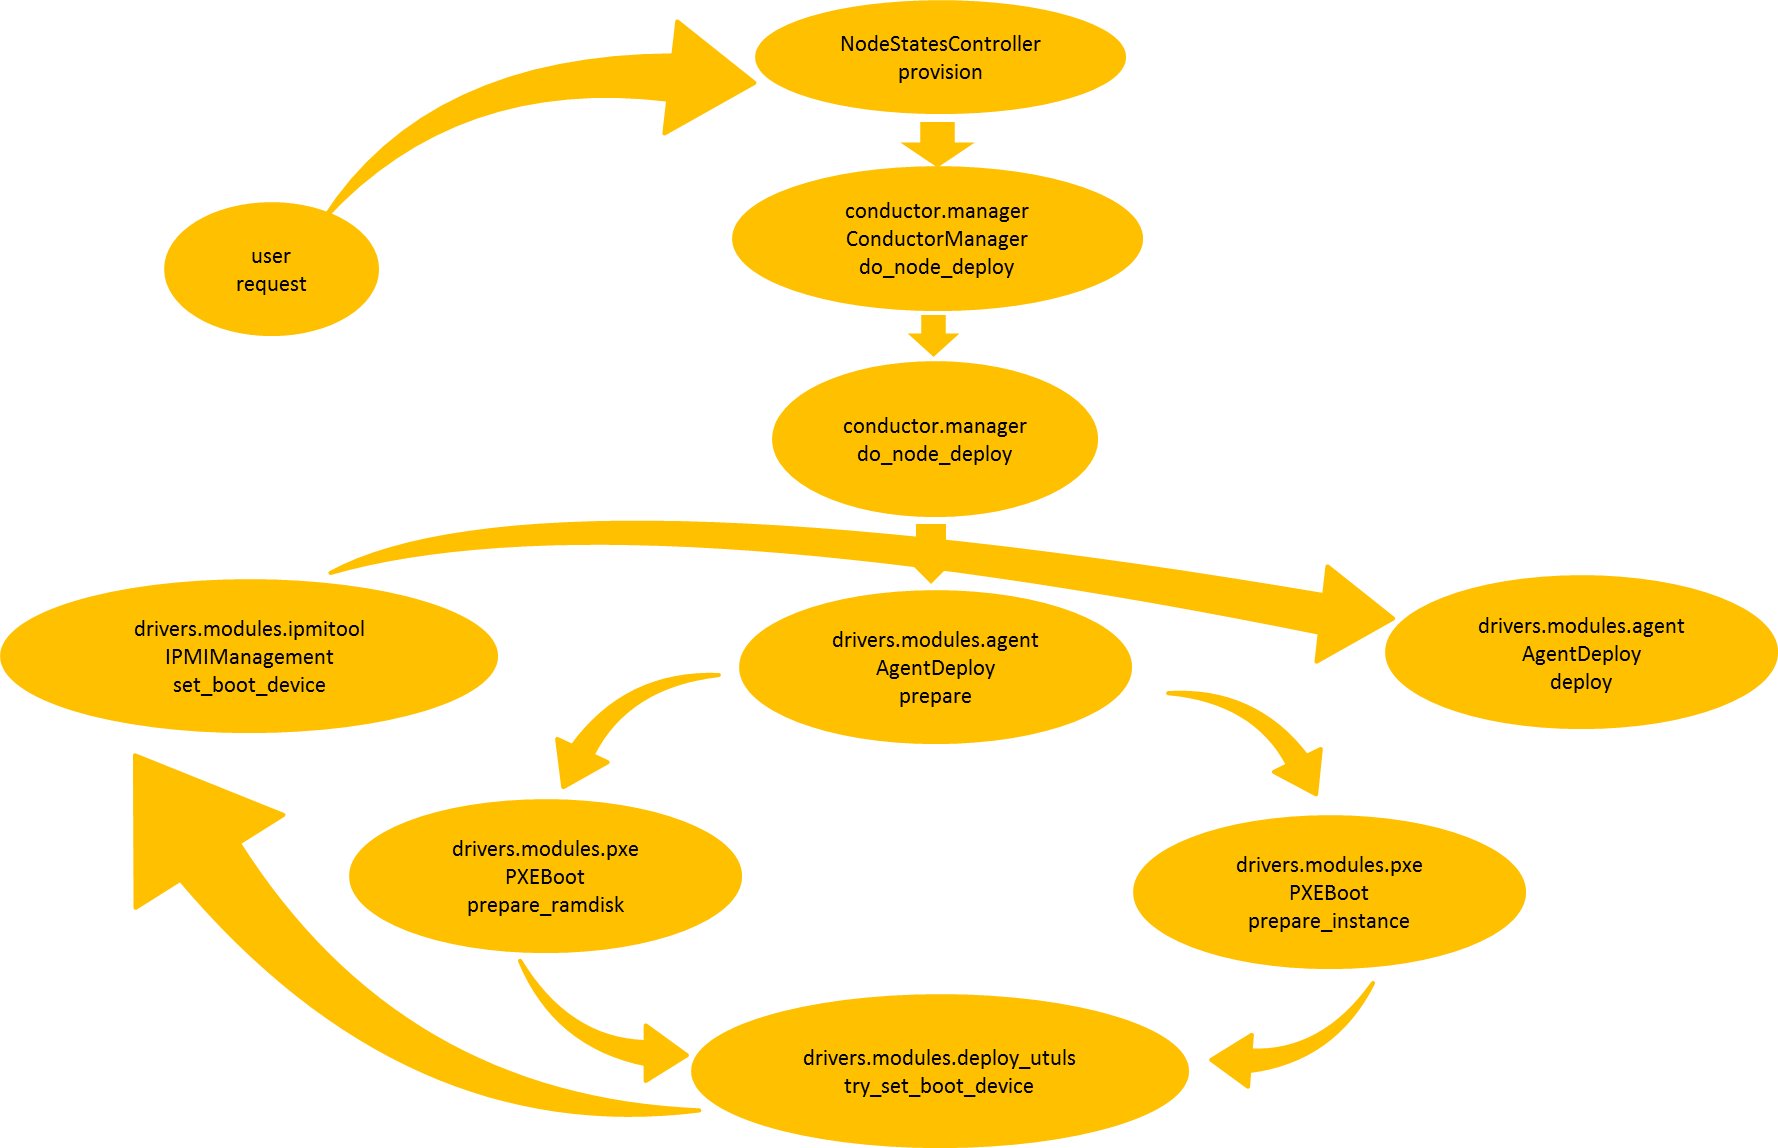
\includegraphics[width=\linewidth]{ironic_workflow1.png}
  \caption{Ironic部署物理机流程一}
  \label{fig:step1}
\end{figure}

而在第二步当中,主要就是依靠ramdisk当中的ipa软件与ironic进行交互,完成剩余的工作。
但是,完成第二个步骤需要有一些前置的条件:
\begin{itemize}
  \item 部署的物理机已经从deploy的ramdisk正常启动
  \item deploy的ramdisk当中预装有ipa(iroinc-python-agent)
  \item ramdisk当中的ipa已经开始正常运行
\end{itemize}

Ipa需要开机运行,其主要的工作有2部分:
\begin{enumerate}
  \item 启动一个http服务,作为服务端,接收ironic的请求
  \item 启动一个heartbeat线程,作为客户端,向ironic发送请求
\end{enumerate}

而ipa和ironic进行交互,完成物理机部署的具体流程如\nameref{fig:step2}所示
\begin{figure}[H]
  \centering
  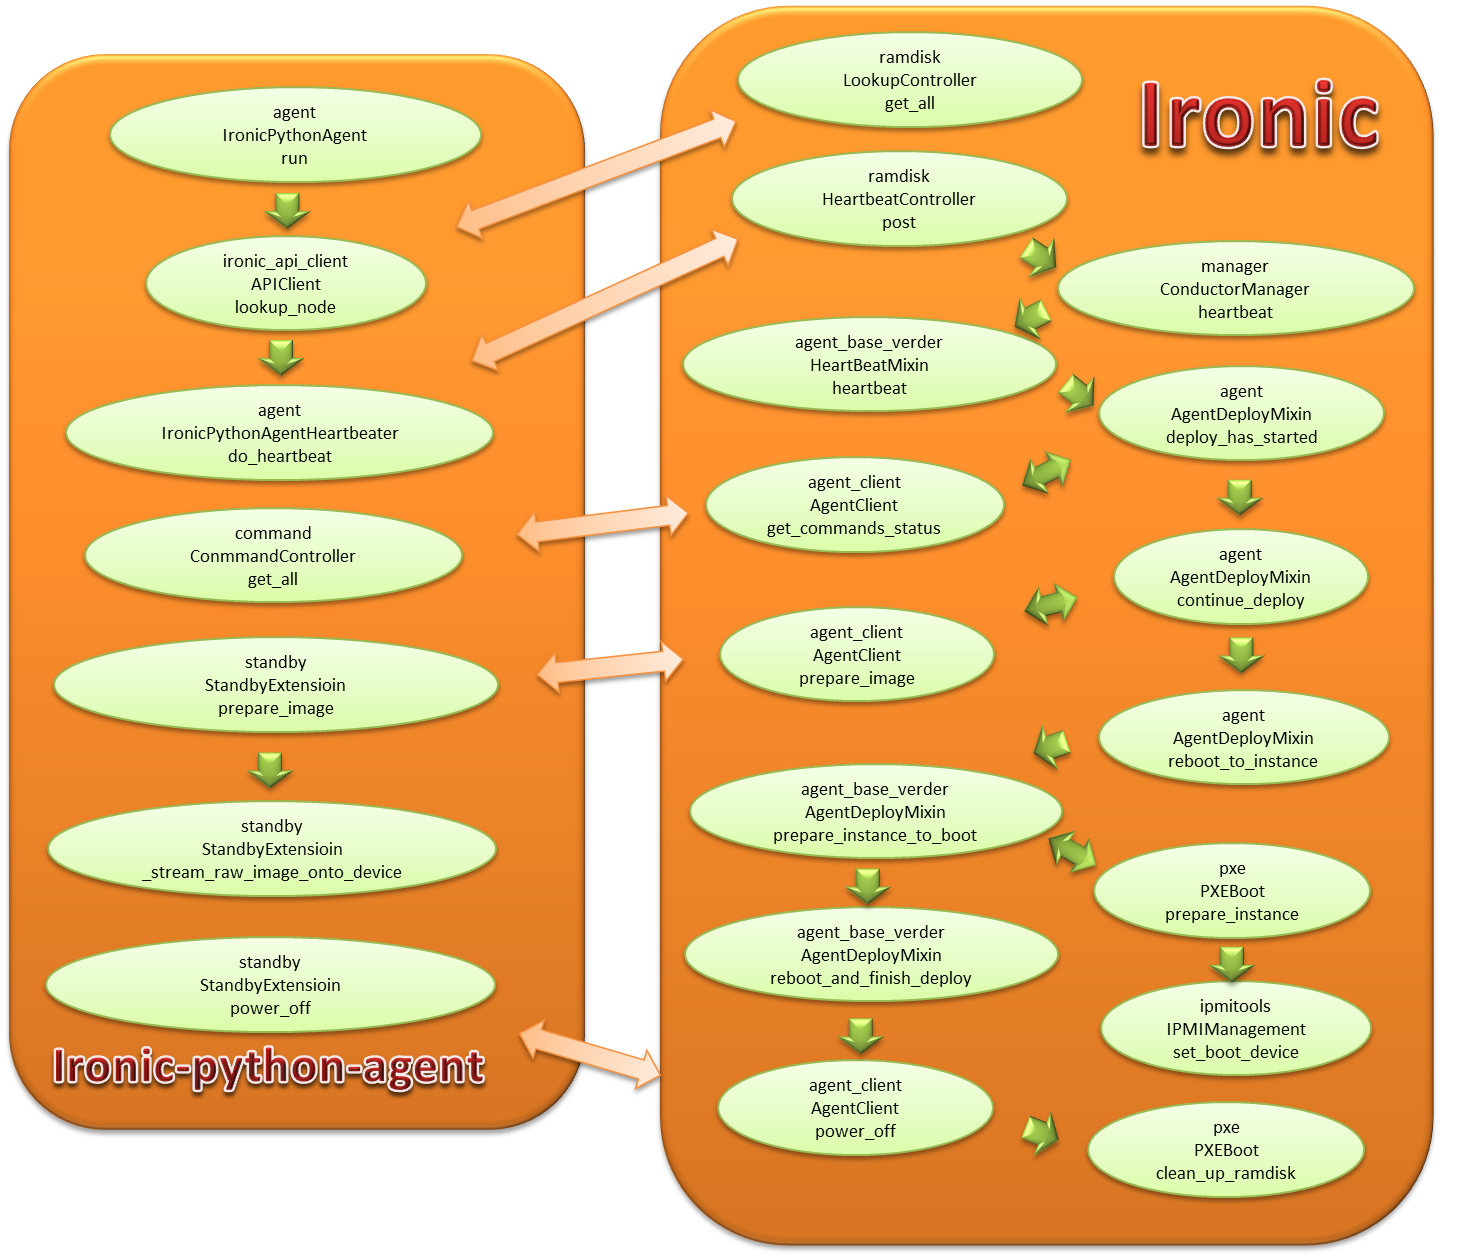
\includegraphics[width=\linewidth]{ironic_workflow2.png}
  \caption{Ironic部署物理机流程二}
  \label{fig:step2}
\end{figure}

\begin{comment}
\begin{tikzpicture}[->,>=stealth',shorten >=1pt,auto,node distance=2.8cm,
                    semithick]
  \tikzstyle{every state}=[fill=yellow1,draw=none,text=black]

  \node[state]         (S) at (-6, 0)              {$S$};
  \node[state]         (xin1) at (-2, 3)           {$X^1_{in}$};
  \node[state]         (xin2) at (-2, 1)        {$X^2_{in}$};
  \node[state]         (xin3) at (-2, -1)       {$X^3_{in}$};
  \node[state]         (xin4) at (-2, -3)           {$X^4_{in}$};
  \node[state]         (xout1) at (0, 3)          {$X^1_{out}$};
  \node[state]         (xout2) at (0, 1)        {$X^2_{out}$};
  \node[state]         (xout3) at (0, -1)   {$X^3_{out}$};
  \node[state]         (xout4) at (0, -3)           {$X^4_{out}$};
  \node[state]         (xin5)  at (3, -2)   {$X^5_{in}$};
  \node[state]         (xout5) at (5, -2)   {$X^5_{out}$};
  \node[state]         (DC) at (7, 2)           {$DC$};

  \path (S) edge[bend left=26]              node {$\infty$} (xin1)
            edge[bend left=12]              node {$\infty$} (xin2)
            edge[bend right=12]             node {$\infty$} (xin3)
            edge[bend right=26]             node {$\infty$} (xin4)
        (xin1) edge  node {$\alpha=1$} (xout1)
        (xin2) edge  node {$\alpha=1$} (xout2)
        (xin3) edge  node {$\alpha=1$} (xout3)
        (xin4) edge  node {$\alpha=1$} (xout4)
        (xin5) edge  node {$1$} (xout5);
  \draw[->] (xout1) to[out=-30,in=150] node {$\beta$} (xin5);
  \draw[->] (xout2.east) to[out=-15,in=165] node [below] {$\beta$} (xin5);
  \draw[->] (xout3.east) to[out=0,in=180] node [below] {$\beta$} (xin5.west);
  \draw[->] (xout1) to[out=-5,in=175] node {$\infty$} (DC);
  \draw[->] (xout5) to[out=40, in=-120] node {$\infty$} (DC);
\end{tikzpicture}
\end{comment}
